\documentclass[a4paper,UTF8]{article}
\usepackage{ctex}
\usepackage[margin=1.25in]{geometry}
\usepackage{color}
\usepackage{graphicx}
\usepackage{amssymb}
\usepackage{amsmath}
\usepackage{amsthm}
\usepackage{soul, color, xcolor}
\usepackage{bm}
\usepackage{tcolorbox}
\usepackage{hyperref}
\usepackage{pythonhighlight}
\numberwithin{equation}{section}
%\usepackage[thmmarks, amsmath, thref]{ntheorem}
\theoremstyle{definition}
\newtheorem*{solution}{Solution}
\newtheorem*{prove}{Proof}
\usepackage{multirow}
\usepackage{diagbox}
\usepackage{float}

\def \X {\mathbf{X}}
\def \A {\mathbf{A}}
\def \w {\hat{\boldsymbol{w}}}
\def \y {\mathbf{y}}
\def \x {\mathbf{x}}
\def \z {\mathbf{z}}
\def \hy {\widehat{y}}
\def \by {\Bar{y}}
\def \H {\mathbf{H}}
\def \I {\mathbf{I}}
\setlength{\parindent}{0pt}
%--

%--
\begin{document}
\title{机器学习导论\ 习题一}
\author{211300044, 吴羽珩, \href{mailto:邮箱}{2559280859@qq.com}}
\maketitle
\section*{作业提交注意事项}
\begin{tcolorbox}
	\begin{enumerate}
		\item[1.] 请在LaTeX模板中第一页填写个人的学号、姓名、邮箱;
		\item[2.] 本次作业需提交作答后的该 pdf 文件、编程题代码(.py文件); {\color{red}\textbf{请将二者打包为~.zip 文件上传}}. 注意命名规则, 三个文件均命名为 “学号\_姓名” + “.后缀” (例如 211300001\_张三” + “.pdf”、“.py”、“.zip”);
		\item[3.] 若多次提交作业, 则在命名~.zip 文件时加上版本号, 例如 211300001\_张三\_v1.zip” (批改时以版本号最高的文件为准);
		\item[4.] 本次作业提交截止时间为 {\color{red}\textbf{ 3 月 29 日23:59:59}}. 未按照要求提交作业, 提交作业格式不正确, {\color{red}\textbf{作业命名不规范}}, 将会被扣除部分作业分数; 除特殊原因 (如因病缓交, 需出示医院假条) 逾期未交作业, 本次作业记 0 分; {\color{red}\textbf{如发现抄袭, 抄袭和被抄袭双方成绩全部取消}};
		\item[5.] 本次作业提交地址为 \href{https://box.nju.edu.cn/u/d/008080744a60484ea526/}{here}, 请大家预留时间提前上交, 以防在临近截止日期时, 因网络等原因无法按时提交作业.
	\end{enumerate}
\end{tcolorbox}
\newpage


\section{[15pts] Derivatives of Matrices}
 有 $\alpha \in \mathbb{R}$, $\y\in \mathbb{R}^{m×1}$, $\x\in \mathbb{R}^{n×1}$, 试完成下题, 并给出计算过程.
\begin{enumerate}
	\item[(1)] \textbf{[4pts]} 此问中假设 $\A\in \mathbb{R}^{n×n}$, 且 $\alpha=\x^\top\A\x$, 试求 $\frac{\partial \alpha}{\partial \x}$.
	\item[(2)] \textbf{[5pts]} 此问中假设 $\A\in \mathbb{R}^{m×n}$, 且 $\alpha=\y^\top\A\x$, 同时 $\y$、$\x$ 为 $\z$ 的函数, 试求 $\frac{\partial \alpha}{\partial \z}$.
	\item[(3)] \textbf{[6pts]} 此问中假设 $\A\in \mathbb{R}^{n×n}$ 且 $\A$ 可逆, $\A$ 为 $\alpha$ 的函数同时 $\frac{\partial \A}{\partial \alpha}$ 已知. 试求 $\frac{\partial \A^{-1}}{\partial \alpha}$.
\end{enumerate}
(提示: 可以参考 \href{https://www.math.uwaterloo.ca/~hwolkowi/matrixcookbook.pdf}{The Matrix Cookbook}.)

\begin{solution}
	此处用于写解答 (中英文均可)\\
	我们有
	\[	
		\frac{\partial(a^T b)}{\partial x}=\frac{\partial a^T}{\partial x}b+\frac{\partial b^T}{\partial x}a
	\]
	\begin{enumerate}
	\item[(1)]
	\[	
		\alpha = \sum_{j=1}^n \sum_{i=1}^n a_{ij}x_y x_j
	\]
	所以对于向量$\x$的第k个元素$x_k$,有偏导数
	\[
		\frac{\partial \alpha}{\partial x_k}=\sum_{j=1}^n a_{kj} x_j + \sum_{i=1}^n a_{ik}x_i
	\]
	由此可得偏导数为:
	\[
		\frac{\partial \alpha}{\partial x}=\ \frac{\partial {(x^T\A x)}}{\partial x}=\frac{\partial x^T}{\partial x}\A x+\frac{\partial x^T \A^T}{\partial x}x =(\A + \A^T)x
	\]
	\item[(2)]
	\[
		\frac{\partial \alpha}{\partial z}=\frac{\partial \alpha}{\partial \x}\frac{\partial \x}{\partial \z}+\frac{\partial \alpha}{\partial \y}+\frac{\partial \y}{\partial \z}=[\frac{\partial y}{\partial z}]^T \A x+[\frac{\partial x}{\partial z}]^T \A^T y
	\]
	\item[(3)]由定义:\ $\A^{-1}\A=\I$\\上式两端对$\alpha$求偏导:
	\[\A^{-1}\frac{\partial \A}{\partial \alpha}+\frac{\partial\A^{-1}}{\partial \alpha}\A=0\]
	 \\所以\[\frac{\partial \A^{-1}}{\partial \alpha}=-\A^{-1}\frac{\partial \A}{\partial \alpha} \A^{-1}\]
	\end{enumerate}
\end{solution}




\newpage
\section{[15pts] Performance Measure}
 性能度量是衡量模型泛化能力的评价标准, 在对比不同模型的能力时, 使用不同的性能度量往往会导致不同的评判结果.
请仔细阅读《机器学习》第二章 2.3.3 节. 在书中, 我们学习并计算了模型的二分类性能度量. 下面我们给出一个多分类 (四分类) 的例子, 请根据学习器的具体表现, 回答如下问题.
\begin{table}[ht]
	\centering
	\caption{类别的真实标记与预测}
	\label{tab:samples1}
	\begin{tabular}{|l|l|l|l|l|}
		\hline
	\diagbox{真实类别}{预测类别}   & 第一类 & 第二类 & 第三类 & 第四类 \\ \hline
	第一类 & 7   & 2   & 1   & 0   \\ \hline
	第二类 & 0   & 9   & 0   & 1   \\ \hline
	第三类 & 1   & 0   & 8   & 1   \\ \hline
	第四类 & 1   & 2   & 1   & 6   \\ \hline
	\end{tabular}
\end{table}
\begin{enumerate}
	\item[(1)] \textbf{[5pts]}  如表~\ref{tab:samples1} 所示, 请计算该学习器的错误率及精度.
	\item[(2)] \textbf{[5pts]}  请分别计算宏查准率, 宏查全率, 微查准率, 微查全率, 并两两比较大小.
	\item[(3)] \textbf{[5pts]}  分别使用宏查准率, 宏查全率, 微查准率, 微查全率计算宏$F1$度量, 微$F1$度量, 并比较大小.

\end{enumerate}

	此处用于写解答(中英文均可)

	\begin{solution}
		~\\(1)学习器的精度为:$\frac{3}{4}=75\%$,\quad 学习器的错误率为 $1-\text{精度}=\frac{1}{4}=25\%$
		~\\(2)四个混淆矩阵:1类,非1类;2类,非2类;3类,非3类;4类,非4类\\
		宏查准率为:
		\[
			\begin{split}
			\text{macro-P}&=\frac{1}{4}(\frac{7}{9}+\frac{9}{13}+\frac{8}{10}+\frac{6}{8})=0.755\\
			\text{macro-R}&=\frac{1}{4}(\frac{7}{10}+\frac{9}{10}+\frac{8}{10}+\frac{6}{10})=0.750
			\end{split}
		\]
		经过计算四个混淆矩阵对应位置元素的平均值后:\\
		$\overline{TP}=7.5$,$\overline{FP}=2.5$,$\overline{FN}=2.5$\\所以有:
		\[
			\text{micro-P}=0.750\\
			\text{micro-R}=0.750
		\]
		~\\由此发现宏查准率大于宏查全率\  微查准率和微查全率相等
		~\\(3)由书上的公式:
		\[
			\begin{split}
			\text{macro-F1}&=0.7525\\
			\text{micro-F1}&=0.7500
			\end{split}
		\]
		宏F1度量大于微F1度量.
	\end{solution}

\newpage

\section{[15pts] ROC \& AUC}
 ROC 曲线与其对应的 AUC 值可以反应分类器在 “一般情况下” 泛化性能的好坏. 请仔细阅读《机器学习》第二章 2.3.3 节,并完成本题.
\begin{table}[ht]
	\centering
	\caption{样例的真实标记与预测}
	\begin{tabular}{c|ccccccccc}
		\hline 样例 & $x_1$ & $x_2$ & $x_3$ & $x_4$ & $x_5$ & $x_6$ & $x_7$ & $x_8$ & $x_9$ \\
		\hline 标记 & 0 & 1 & 0 & 1 & 0 & 0 & 1 & 1 & 0 \\
		\hline 分类器输出值 & 0.4 & 0.9 & 0.7 & 0.4 & 0.2 & 0.8 & 0.8 & 0.6 & 0.5 \\
		\hline
	\end{tabular}
	\label{tab:samples}
\end{table} 
\begin{enumerate}
    \item[(1)] \textbf{[5pts]}  如表~\ref{tab:samples} 所示, 第二行为样例对应的真实标记, 第三行为某分类器对样例的预测结果. 请根据上述结果, 绘制分类器在该样例集合上的 ROC 曲线, 并写出绘图中使用到的节点 (在坐标系中的) 坐标及其对应的阈值与样例编号.
    \item[(2)] \textbf{[3pts]}  根据上题中的 ROC 曲线, 计算其对应的 AUC 值(请给出具体的计算步骤).
    \item[(3)] \textbf{[7pts]}  结合前两问使用的例子(可以借助图片示意), 试证明对有限样例成立:
    \begin{equation}
        \label{eq:auc}
            \text{AUC} = \frac{1}{m^+m^-}\sum_{x^+\in D^+}\sum_{x^-\in D^-}\left(\mathbb{I}\left\{f(x^+) > f(x^-)\right\}+\frac{1}{2}\mathbb{I}\left\{f(x^+)=f(x^-)\right\}\right).
    \end{equation}    
\end{enumerate}

\begin{figure}[H]
	\centering%居中
	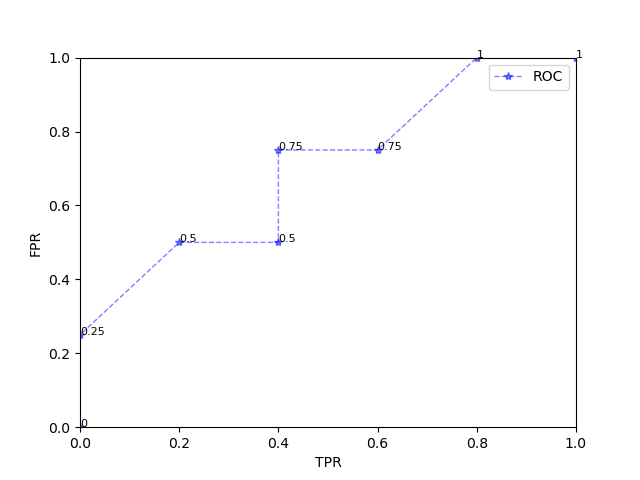
\includegraphics[width=1\textwidth]{myplot.png}
	\caption{ROC曲线图}
\end{figure}
\begin{solution}
此处用于写解答(中英文均可)
~\\(1)阈值与对应的样例编号分别为:
\begin{table}[ht]
	\centering
	\begin{tabular}{c|cccccccc}
		\hline 样例 & NULL & $x_2$ & $x_7,x_7$ & $x_3$ & $x_8$ & $x_9$ & $x_1,x_4$ & $x_5$\\
		\hline 阈值 & 1 & 0.9 & 0.8 & 0.7 & 0.6 & 0.5 & 0.4 & 0.2  \\
		\hline
	\end{tabular}
\end{table} 
~\\(2)\ AUC的值即为上述ROC曲线与x轴所围成的面积:
	\[
		\begin{split}
		S &=\frac{1}{2} \sum_{i=1}^8(x_{i+1}-x_i)(y_i+y_{i+1})\\
		&=0.7
		\end{split}
	\]
~\\(3)\ 注意到AUC的物理意义为正样本预测结果大于负样本预测结果的概率,他反映了分类器对于样本的排序能力,换言之,就是随机拿出一个正样本和一个负样本,正样本的预测结果比负样本的预测结果大的概率:如果我们把所有的正样本和负样本都比较一遍,那么按照题干,正样本有$m_+$个,负样本有$m_-$个,那么一共有$m_+ * m_-$对,而题干中的双重求和符号(可以理解为双重循环)即遍历每一对,统计正样本预测值大于负样本预测值的一共有多少对,值得注意的是,对于正样本预测值等于负样本预测值的情况记为0.5,所以我们得到了题干中的公式\[\text{AUC} = \frac{1}{m^+m^-}\sum_{x^+\in D^+}\sum_{x^-\in D^-}\left(\mathbb{I}\left\{f(x^+) > f(x^-)\right\}+\frac{1}{2}\mathbb{I}\left\{f(x^+)=f(x^-)\right\}\right)\]
计算证明:在 ROC 曲线当中,每条横线都对应着至少一个标签为反例的样本,同样,每条垂线都对应着至少一个标签为正例的样本,斜线则对应着多个预测值相同的正或反样本.每增加一个正例,在ROC图中y轴的投影长度为$\frac{1}{m^+}$,每增加一个负例,在x轴的投影长度为$\frac{1}{m^-}$
所以对于某一个梯形来说
\[
	\begin{split}
	S&=\frac{1}{2}(x_{i+1}-x_i)\big[\sum_{x^+\in D^+}( \frac{2}{m^+}\mathbb{I}\left\{f(x^+) > f(x^-)\right\}+\frac{1}{m^+}\mathbb{I}\left\{f(x^+) = f(x^-)\right\} ) \big]\\
	&=\frac{1}{m^+m^-}\sum_{x^+\in D^+}\left(\mathbb{I}\left\{f(x^+) > f(x^-)\right\}+\frac{1}{2}\mathbb{I}\left\{f(x^+)=f(x^-)\right\}\right)
	\end{split}
\]
所以所有梯形的面积和为AUC的值,即为:\[
	\text{AUC} = \frac{1}{m^+m^-}\sum_{x^+\in D^+}\sum_{x^-\in D^-}\left(\mathbb{I}\left\{f(x^+) > f(x^-)\right\}+\frac{1}{2}\mathbb{I}\left\{f(x^+)=f(x^-)\right\}\right)
\]
\end{solution}
\newpage




\section{[20pts] Linear Regression}
 线性回归模型是一类常见的机器学习方法, 其基础形式与变体常应用在回归任务中. 根据《机器学习》第三章 3.2 节中的定义, 可以将收集到的 $d$ 维数据及其标签如下表示: 

\[
\X=\left(\begin{array}{ccccc}
x_{11} & x_{12} & \ldots & x_{1 d} & 1 \\
x_{21} & x_{22} & \ldots & x_{2 d} & 1 \\
\vdots & \vdots & \ddots & \vdots & \vdots \\
x_{m 1} & x_{m 2} & \cdots & x_{m d} & 1
\end{array}\right)
=
\left(\begin{array}{cc}
\x_1^{\top} & 1 \\
\x_2^{\top} & 1 \\
\vdots & \vdots \\
\x_m^{\top} & 1
\end{array}\right)
;\quad \y 
=
\left(\begin{array}{c}
y_1\\
y_2\\
\vdots\\
y_m
\end{array}\right).
\]

将参数项与截距项合在一起, 定义为$\w=
\left(
\boldsymbol{w}^\top; b\right)^\top$. 此时成立 $\hat{\y} = \X\w$.《机器学习》式 (3.11) 给出了最小二乘估计 (Least Square Estimator, LSE) 的闭式解: 
\begin{equation}
    \label{eq:LSE}
    \w_{\textbf{LSE}}^* = \left(\X^\top\X\right)^{-1}\X^\top\y.
\end{equation}
  
\begin{enumerate}
\item[(1)] \textbf{[8pts]} (投影矩阵的性质) 
% 在得到 $\w^*$ 后,可使用 $\mathbf{\hy} = \X \w^*$ 得到样本标记的预测值.
容易验证, 当采用最小二乘估计 $\w_{\textbf{LSE}}^*$ 时, 成立: 
\begin{equation*}
    \mathbf{\hy} = \X \w_{\textbf{LSE}}^* = \X\left(\X^\top\X\right)^{-1}\X^\top\y.
\end{equation*}

记 $\H = \X\left(\X^\top\X\right)^{-1}\X^\top$, 则有 $\mathbf{\hy} = \H\y$. $\H$ 被称为 “Hat Matrix”, 其存在可以从空间的角度, 把 $\mathbf{\hy}$ 看作是 $\y$ 在矩阵 $\H$ 空间中的投影. $\H$ 矩阵有着许多良好的性质.
已知此时 $\X$ 矩阵列满秩, $\I$ 为单位阵, 试求 $\I - \H$ 的全部特征值并注明特征值的重数.
% \begin{center}
% \fcolorbox{gray}{gray!10}{\parbox{.85\linewidth}{背景: 记 $\H = \X\left(\X^\top\X\right)^{-1}\X^\top$,则有$\mathbf{\hy} = \H\y$.\\$\H$ 被称为“Hat Matrix”,其存在可以从空间的角度,把 $\mathbf{\hy}$ 看作是 $\y$ 在矩阵 $\H$ 空间中的投影.$\H$ 矩阵有着许多良好的性质.}}
% \end{center}

(提示: 利用 $\H$ 矩阵的投影性质与对称性.)



\item[(2)] \textbf{[5pts]} (岭回归) 当数据量 $m$ 较小或数据维度 $d$ 较高时, 矩阵 $\X^\top\X$ 可能不满秩, \ref{eq:LSE} 中的取逆操作难以实现. 此时可使用岭回归代替原始回归问题, 其形式如下: 
\begin{equation}
    \label{eq:Ridge}
    \w_{\textbf{Ridge}}^* = \mathop{\arg\min}_{\w} \frac{1}{2}\left(\lVert \y - \X \w \rVert_2^2 +\lambda \lVert \w \rVert_2^2\right).
\end{equation}
试求岭回归问题的闭式解, 并简述其对原问题的改进.

\item[(3)] \textbf{[7pts]} 定义 $\Tilde{\x}_i = \left(\x_i^\top;1\right)^\top$,
$\hy_i = \Tilde{\x}_i^\top \w_{\textbf{LSE}}^*$,
$\by = \frac{1}{m} \sum\limits_{i=1}^m y_i $. 

对线性回归模型进行统计分析时,会涉及如下三个基础定义: 
\begin{equation*}
    \left\{
        \begin{aligned}
        &\text{Total sum of squares (SST): }& &\sum\limits_{i=1}^m\left(y_i-\by\right)^2 \\
        &\text{Regression sum of squares (SSR): }& &\sum\limits_{i=1}^m\left(\hy_i-y_i\right)^2 \\
        &\text{Residual sum of squares (SSE): }& &\sum\limits_{i=1}^m\left(\hy_i-\by\right)^2
        \end{aligned}
    \right.
\end{equation*}

试证明 SST = SSR + SSE. (提示: 使用向量形式可以简化证明步骤.)



\end{enumerate}


\begin{solution}
此处用于写解答(中英文均可)
~\\(1)由于\[\H^T=\H,\H^2=\H\]我们得知$H$矩阵是一个对称幂等矩阵,同理\[(\I-\H)^T=\I-\H,(\I-\H)^2=\I-\H\]可知$\I-\H$也是一个对称幂等矩阵.我们先看$\H$矩阵,利用对称幂等矩阵的性质可知(特征值的定义易证),\ $\H$矩阵的特征值为1,0.\\ $\H$是一个$m\cdot m$的矩阵,设$\H$矩阵的秩为$r(\H)$,则特征值1的重数为$r(\H)$,特征值0的重数为$m-r(\H)$,下求$r(\H)$:\\由于矩阵$\X$是一个列满秩的矩阵,所以$r(\X)=d+1$,由矩阵秩的性质$r(\X^T \X)=r(\X)=d+1$且$\X^T \X$是一个$(d+1)\cdot (d+1)$的矩阵,所以$\X^T \X$是一个方阵且可逆,又由于$\X^T$行满秩,$\X$列满秩,所以\[\H=\X(\X^T \X)^{-1}\X^T\]的秩为$d+1$\\所以$\I-\H$的特征值为0(重数为d+1),\quad 1(重数为m-d-1)\\
~\\(2)设\[L(w)=(\X w-y)^T(\X w-y)+\lambda w^T w\] 我们要求$\w$\ minimize\ $L(w)$,求\[\frac{\partial L(w)}{\partial w}=2\X^T \X w-2\X^T Y+2\lambda Ew\] 另其为0,解得\[w=(\X^T \X+\lambda E)^{-1} \X^T y\]\\岭回归也是一种线性回归,只不过在算法建立回归方程的时候加上正则化的限制,从而达到解决过拟合的效果,通过放弃最小二乘法的无偏性,以损失部分信息、降低精度为代价获得回归系数更为符合实际、更可靠的回归方法,对病态数据的拟合要强于最小二乘法。\\
~\\(3)将左侧SST变为\[\sum\limits_{i=1}^m\left(y_i-\hy_i+\hy_i-\by\right)^2\] 经过化简整理得:要证明$SST=SSE+SSR$\ ,只须证\[\sum(\hy_i-\by_i)(y_i-\hy_i)=0\]  最小二乘法的原理为将误差的平方和最小化,  令\[\hy_i=\beta_0+\beta_1x_i\]则\[ S=\sum(y_i-\hy_i)^2=\sum(y_i-\beta_0-\beta_1x_i)^2\] 我们就是要找到$\beta_0,\beta_1$使S最小.
令\[\frac{\partial S}{\partial \beta_0}=0\]化简后得到\[\sum{y_i-\hy_i}=0 \quad, (1)\]我们再求\[\frac{\partial S}{\partial \beta_1}=0\]化简后可以得到\[\sum x_i(y_i-\hy_i)=0\]又因为\[\hy_i=\beta_0+\beta_1x_i\]所以将\[x_i=\frac{1}{\beta_1}(\hy_i-\beta_0)\]带入上面的方程式整理得\[\frac{1}{\beta_1}\sum\hy_i(y_i-\hy_i)-\frac{\beta_0}{\beta_1}\sum\hy_i(y_i-\hy_i)=0\]  由(1)可知第二项为0,所以我们得到\[\sum\hy_i(y_i-\hy_i)=0 \quad, (2)\]最终根据$(2)-\by*(1)$可得\[ \sum(\hy_i-\by_i)(y_i-\hy_i)=0\]证毕.
\end{solution}

\newpage
\section{[35pts] Logistic Regression in Practice}
对数几率回归 (Logistic Regression, 简称LR) 是实际应用中非常常用的分类学习算法.
\begin{enumerate}
    \item[(1)]  \textbf{[30pts]} 请编程实现二分类的 LR, 要求采用牛顿法进行优化求解. 详细编程题指南请参见链接: \href{https://www.lamda.nju.edu.cn/ML2023Spring/homework/hw1/hw1-code.html}{here}. 请将绘制好的 ROC 曲线放在解答处, 并记录模型的精度与 AUC (保留4位小数).
    \item[(2)]  \textbf{[5pts]} 试简述在对数几率回归中, 相比梯度下降方法, 使用牛顿法的优点和缺点.
\end{enumerate}

\begin{solution}
此处用于写解答 (中英文均可)
~\\
%%%% use following code to insert the picture %%%%%
(1) 
\begin{figure}[H]
\centering
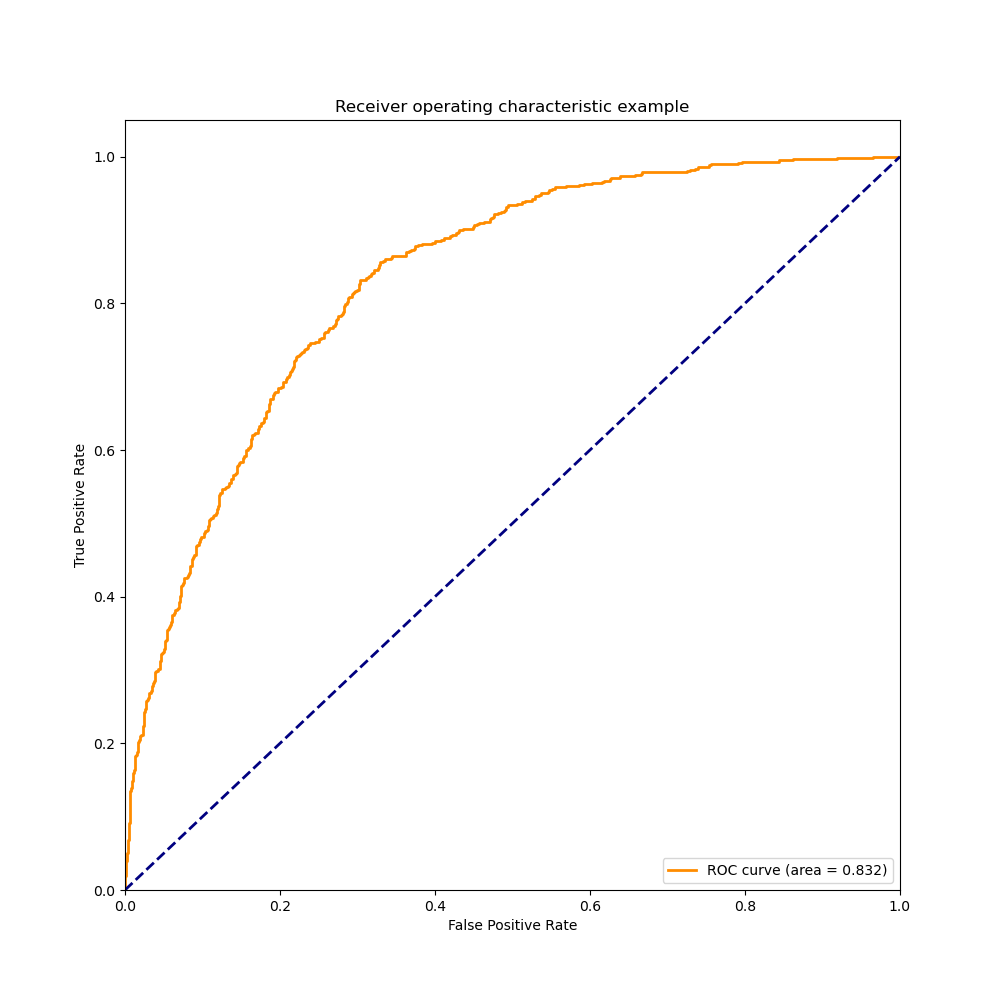
\includegraphics[width=\textwidth]{roc.png}\\
\caption{ROC of test set}
\label{fig:roc}
\end{figure}

Accuracy in test set: 0.7621\\
AUC in test set: 0.8323\\
(2)
牛顿法是通过求解目标函数的一阶导数为0时的参数,进而求出目标函数最小值时的参数。\\
优点:收敛速度很快,hessian矩阵的逆在迭代过程中不断减小,可以起到逐步减小步长的效果。\\
缺点:hessian矩阵的逆计算复杂,代价比较大。牛顿法是局部收敛的.\\
梯度下降法:对于凸函数问题可以全局最优,但是收敛速度比较慢

\end{solution}


\end{document}